\documentclass[12pt,twoside,letterpaper]{article}

\topmargin -0.25cm
\textwidth 15.5cm
\textheight 23cm
\oddsidemargin 0.5cm
\evensidemargin 0.5cm


%\usepackage{epsfig,rotating}
\usepackage{amssymb}
\usepackage{amsmath}
\usepackage{graphicx}
\usepackage{epstopdf}
\usepackage{verbatim}

%\usepackage{doublespace}

%\usepackage{setspace}
%\setstretch{1.667}

%\usepackage{lineno}
%\linenumbers

\begin{document}

\vspace*{-3.5cm}
\begin{flushright}
Version 1a\\
\today
\end{flushright}

%\vspace{0.25in}

\begin{center}
  \begin{large}
  {\bf Pi/K Separation in a Granular Fast-Timing Calorimeter}
  \end{large}
\end{center}

%\vspace{0.25in}

\begin{center}
Evan Angelico and Todd Seiss\\
\emph{University of Chicago and the Institute of High Energy Physics}
\end{center}

\begin{abstract}
This is a note that describes a portion of the work performed from June 14-27th of 2017 at a U. of Chicago/CEPC collaborative workshop. The goal was to learn what the separation power of pions and kaons could be using time of flight and the present conceptual design of the CEPC detector. By scanning the phase space of pixel timing resolution and initial particle momentum, we produced an algorithm dependent measure pion/kaon separation. 
\end{abstract}


\vspace{0.1in}



\section{Introduction}

\section{Shower structure and simulation}

\section{Algorithms}

The power of pion/kaon separation is a function of the reconstruction algorithm used, just as it is a function of particle momentum and pixel timing resolution. 

Two approaches were taken to designing an identification algorithm: one approach does not explicitly use the spatial structure of the calorimeter shower, and the other does attempt to use information from the shower structure. Both algorithms rely heavily on timing information provided by the granular calorimeter pixels. 

\subsection{The ``simple'' algorithm}

The ``simple'' algorithm uses the time and space coordinates of the first few hits in the calorimeter to determine if the particle is arriving too early to be a kaon. As the pion has a lighter mass, particles that arrive early and continue to propagate faster than a kaon are identified as pions, or ``not-kaons''. 

The procedure of the algorithm is as follows:


\begin{enumerate}
\item Assume that the particle that made a shower is a kaon with mass $m_K = 493.7$MeV. Given the momentum of the particle (from the tracker), this constrains the velocity of the particle to be $v_K$. 
\item Given each time and space coordinate of pixel hits in the calorimeter, compute the ``vertex time'',\\
\begin{align}
T^{0}_{i} = t^{\texttt{hit}}_{i} - \frac{r_i}{v_K}
\end{align}
where $r_i = \sqrt{x_i^2 + y_i^2 + z_i^2}$ and $t_i$ is the time measured by the hit pixel. 
\item Make a cut that selects the earliest pixel hits (see Figure ***). This step ensures that the slow component of the shower, secondary particles for example, are not included to compute the average vertex time. 
\item Average the early vertex times that passed the timing cut
\item Compare this average $T^0$ with $T = 0$. If the vertex time deviates significantly from zero, than this particle must not have been a kaon with the given momentum. 
\end{enumerate}

A key parameter in this reconstruction algorithm is the time cut window. This cut determines how many points are used to find the average $T^0$ for a given event. 

An informed decision about the cut value can be made by looking at the timing structure of an entire data set of 1,000 events. Figure \ref{timedist_nosmear} shows that for perfect timing resolution, the fast component of a 5GeV kaon shower has most of its $T^0$ values within 5-10 ps of the first hit time. As this same data sample is smeared by 50 ps timing resolution, the distribution widens and the fast component is spread over about 100ps from the first hit time. 

\begin{figure}[h!]
\centering
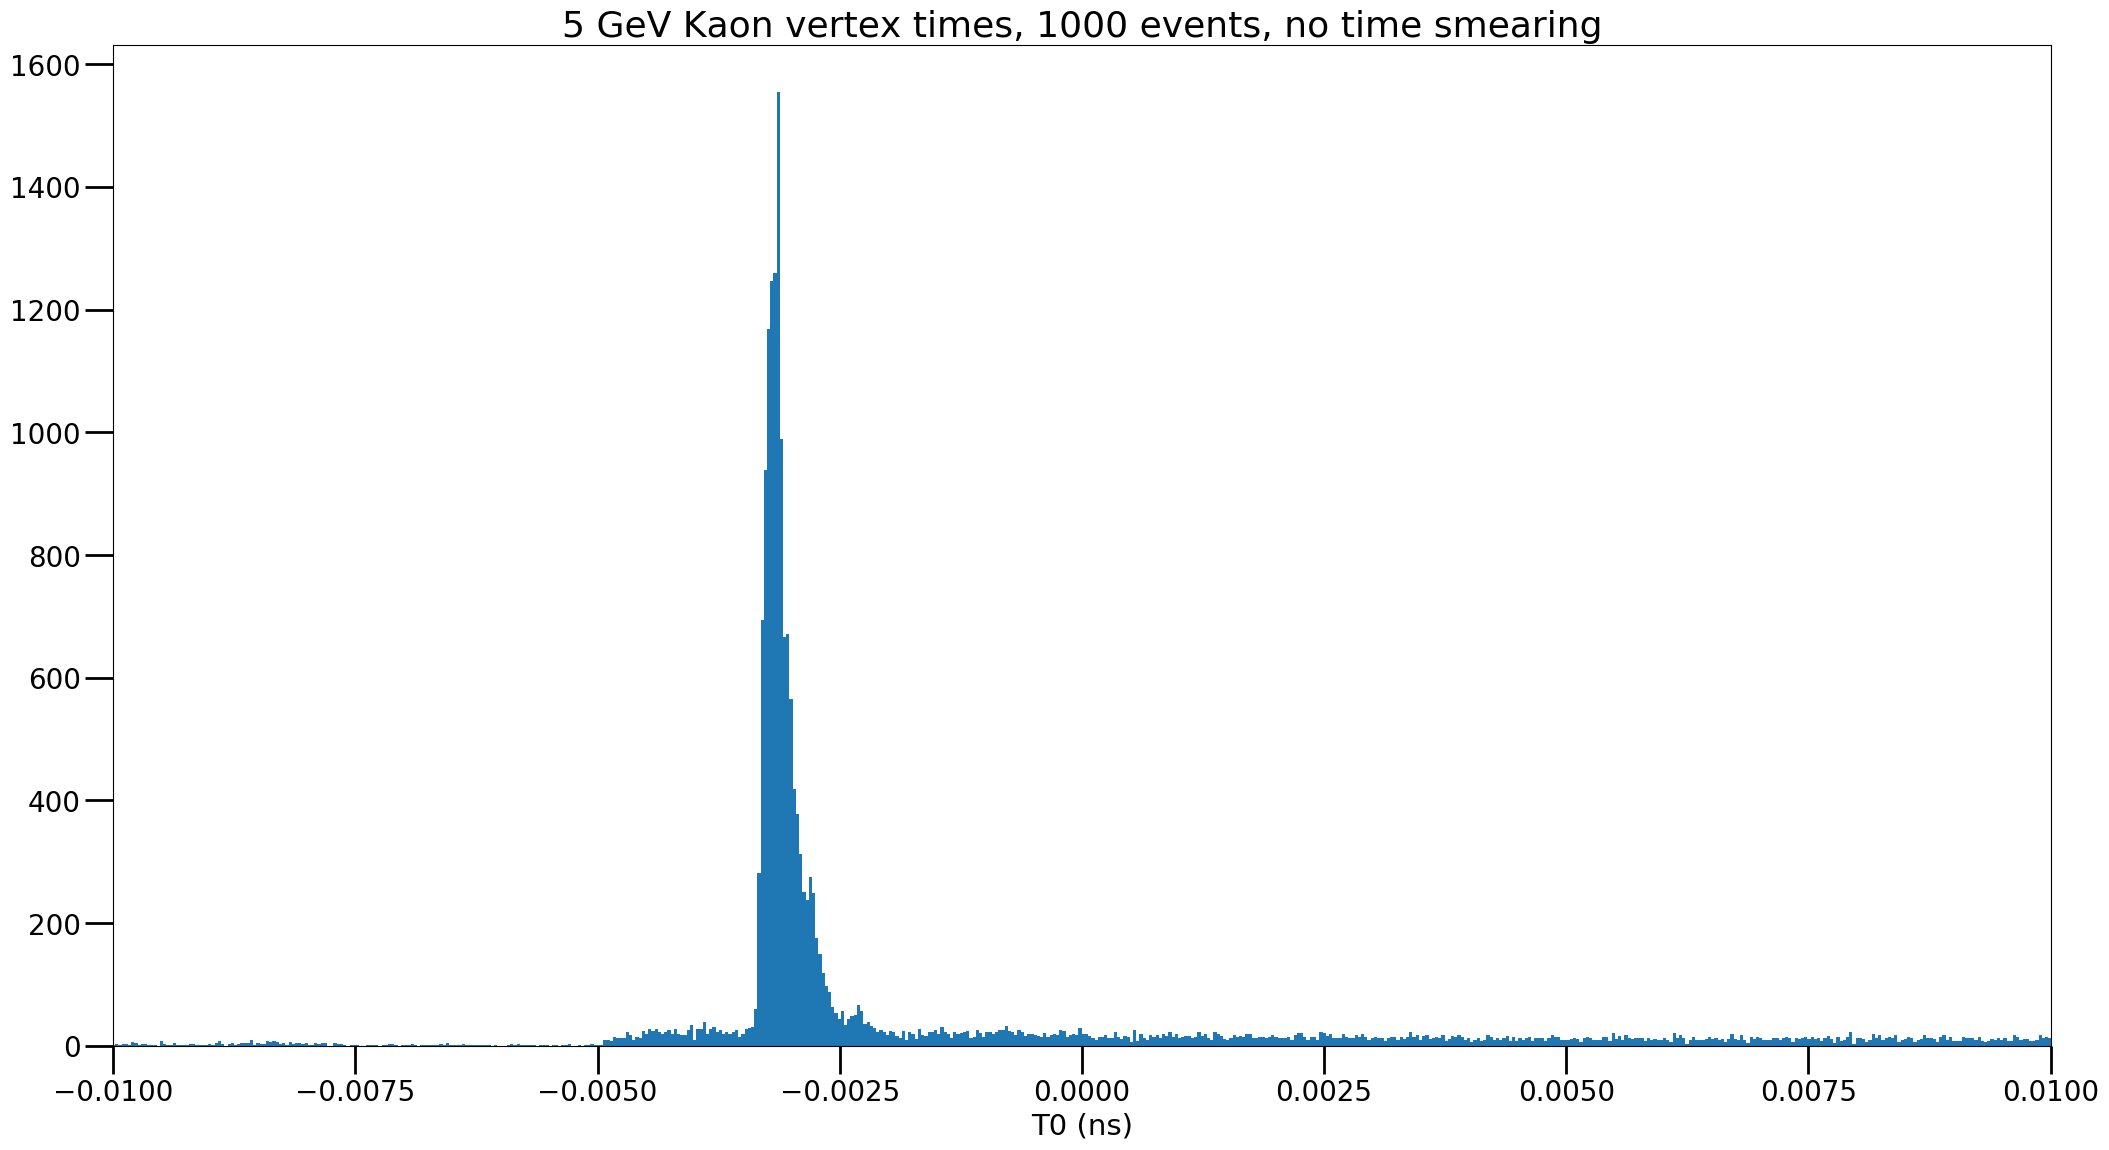
\includegraphics[width=\textwidth]{images/timedist_nosmear.png}
\caption{This plot shows the vertex time $T_i ^0$ for each hit point in a data set of 1000 5GeV kaons. There is no time smearing in this plot. The fast component in the shower is seen as a large peak around 0 with a width of 5-10ps. For this data set, one would want to average only the vertex times calculated within this 5-10ps time cut window.}\label{timedist_nosmear}
\end{figure}

\begin{figure}[h!]
\centering
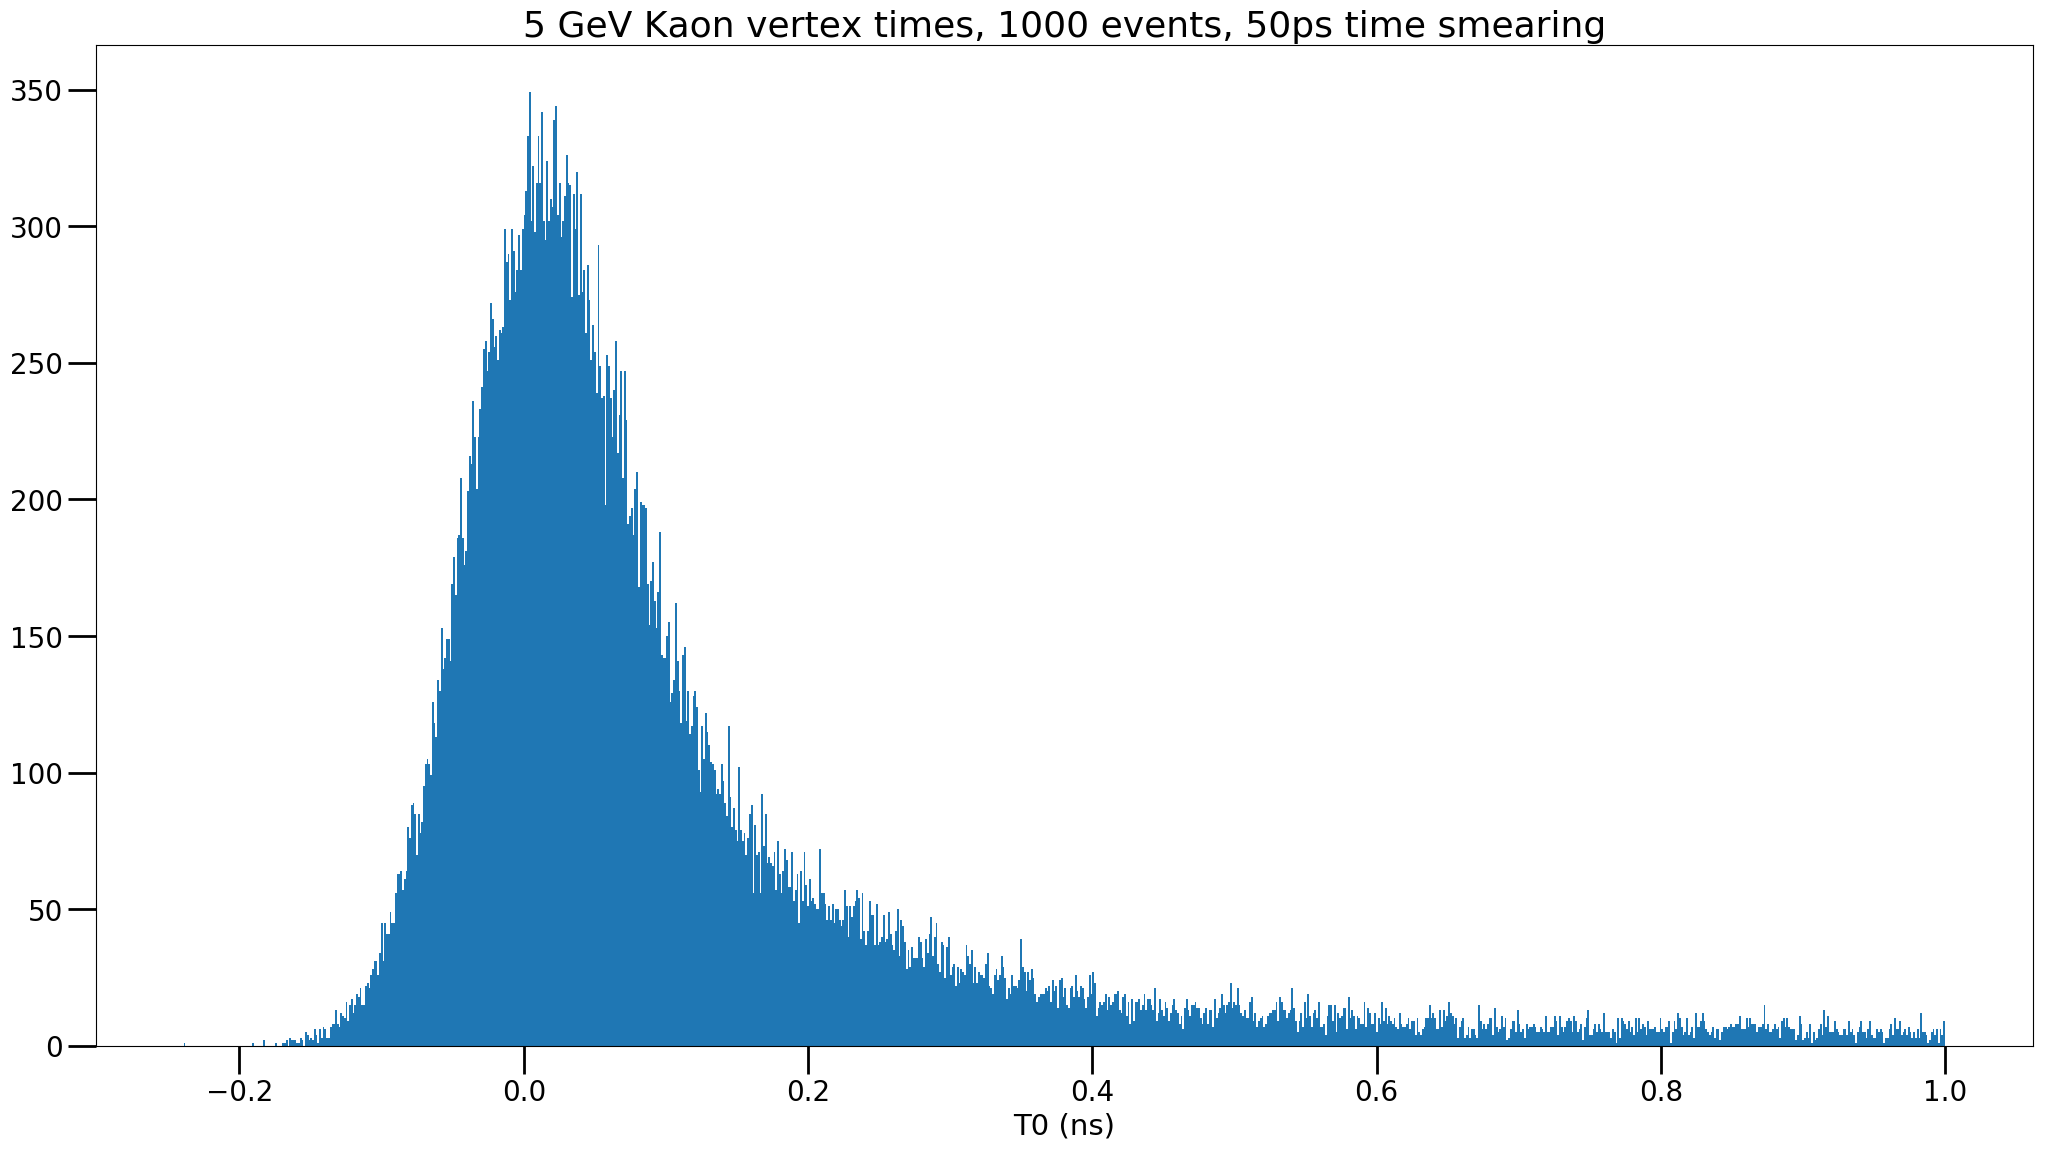
\includegraphics[width=\textwidth]{images/timedist_50ps.png}
\caption{This plot shows the vertex time $T_i ^0$ for each hit point in a data set of 1000 5GeV kaons. There is 50ps pixel time smearing in this plot. Compared to Figure \ref{timedist_nosmear}, the timing distribution of the shower looks more gaussian and has a larger width. The cut window for keeping vertex times should be adjusted appropriately to maximize the number of points used in the average per event.}\label{timedist_smear}
\end{figure}


For testing this algorithm, we used a time-cut equal to the time smearing value. If the time smearing value was less than 7ps, we used 7ps as the time cut. This choice is somewhat arbitrary and should be reconsidered and studied more carefully in the future (section **). We also required that at least 15 hit-points be present in the event as a whole after making a rough cut to reject late neutrons and points outside of the shower region of interest.

Once a time cut has been made on a single event, the remaining vertex times are averaged and the resulting time value falls into one of two distributions: a distribution centered around zero or a distribution offset from zero. The two distributions formed by running the simple algorithm on pions and kaons is shown in Figure ***. Here, one can make out the difference by eye between the reconstructed vertex times of the two particle species. 


A note for future projects: we saw that even the kaon distributions that should be centered around $T^0 = 0$ were shifted, sometimes as much as 300ps depending on particle momentum. We believe that this is a bug or misunderstanding in the simulation, but could be a bug in the reconstruction as well. It does not affect the algorithm as it stands, as one only needs to separate the two distributions. It will affect the algorithm if a more sophisticated time cut is developed that selects hit-points within a time window about 0 instead of selecting hit-points that come less than 5 ps after the earliest hit point. 


\subsection{The ``snake'' and ``highway'' algorithms}

The ``snake'' and ``highway'' algorithms are examples of our first attempt to use spatial information from the the shower. There is a wealth of information in the complex structure of the hadronic shower that may be used to point back to the time of arrival of the particle at the calorimeter. 

These algorithms were built on the principle that the central spatial core of the shower is the fastest component and also the part of the shower that points most accurately to the arrival position/time of the particle. The core of the shower consists of either (1) the original particle or (2) highly forward scattered secondaries that contain a large fraction of the momentum from the original particle. Therefore, the best reconstruction of the entry time of the particle can be made by considering just this portion of the shower and ignoring the secondaries that are surrounding. 


The procedure of both ``snake'' and ``highway'' algorithms is as follows:
\begin{enumerate}
\item Determine the central axis of the shower and the position of the entry point in the calorimeter based on information from the tracker system. 
\item Form a rod of radius $r$ about the central axis, and cut all hit-points that fall outside of this rod
\item For each hit-point that passed the cut, determine a ``rod depth'' defined by the distance of the hit-point from the entry point of the calorimeter, parallel to the shower axis (see Figure **)
\item Fit a line to the distribution of hit-times verses rod depths. The time intercept of this line at depth $=$ 0 is the entry time of the particle into the calorimeter. The entry times then separate the particle species into two mass groups based on early or late arrival at the calorimeter. 
\end{enumerate}

For our data sample, we had particles going directly up the y-axis from the interaction point, and thus they were perpendicular to the calorimeter inner radius. 

A critical parameter of these algorithms is the radius of the rod that selects out the core of the shower. We found that the reconstruction performance was not largely affected by this parameter and decided to arbitrarily set it to $r = $1.5 cm. In the future, this needs to be characterized and set more thoughtfully. 

Any events that had less than 8 hit-points pass the rod cut were not considered for reconstruction. This contributes to the low efficiency of these two algorithms compared to the simple algorithm, which reconstructs almost 95\% of generated events. The ``snake'' and ``highway'' algorithms typically choose to reconstruct 60\% of all events. This number depends heavily on initial particle momentum and time smearing (see section *** for detailed efficiencies).

The two algorithms ``snake'' and ``highway'' differ only in the manner in which they fit a line to the time verses shower depth distribution. These methods are described in the following subsections. A few examples of time verse depth distributions are shown in Figures *** *** ***.

\subsubsection{Snake line fit}

The snake fit procedure is as follows:

\begin{enumerate}
\item Starting from the set of hit-points that pass the rod cut, fit a line to the three earliest hit-points using linear least squares. Record the time-intercept of the fit
\item Add another point to the set of points being fitted, and do another linear least squares fit. Record the time-intercept. 
\item If the difference between the new time-intercept and the most recent previous time-intercept is larger than some value $t_{\texttt{cut}}$, then remove this hit-point from the set of points being fitted and continue with the next hit-point ordered in time. Otherwise, repeat from step 2. 
\end{enumerate}

Therefore, this fitting procedure attempts to add as many points that are close to the time-intercept value of the earliest hit-points, without adding points that are clearly not following the linear distribution. An example of the result of this algorithm is shown in Figure ***. 

The parameter that determines the effectiveness of the fitting algorithm is the value of $t_{\texttt{cut}}$. This cut value determines how strictly to reject bad hit-points and also when the fitting algorithm terminates, i.e. how many points end up being used in the final fit. 

In total, the snake algorithm has the following arbitrary parameters that need to be studied:
\begin{itemize}
\item The differential time cut value $t_{\texttt{cut}}$
\item The radius of the rod cut
\item The minimum number of points needed to pass the rod cut
\item The minimum number of points needed to be used in the final fit
\end{itemize}

The values that we used in our tests are given in Table **, and were chosen based on looking by eye at how well random events were fitting. 

\begin{table}[h!]
\begin{tabular}{|l|l|}\hline\hline
\textbf{parameter} & \textbf{value used in this test} \\ \hline
The differential time cut value $t_{\texttt{cut}}$ & $1.5\times\sigma_t / \sqrt{n}$ \\ \hline
The radius of the rod cut & 1.5 cm \\ \hline
The minimum number of points needed to pass the rod cut & 8 \\ \hline
The minimum number of points needed to be used in the final fit & 8 \\ \hline
\end{tabular}
\caption{Table of parameters used for this fitting algorithm. For the time cut, $\sigma_t$ is the pixel time resolution and $n$ is the number of points currently being used in the fit. If the time resolution was less than 50 ps, $t_{\texttt{cut}} = 50\texttt{ps} / \sqrt{n}$. }\label{snake_params}
\end{table}


\subsubsection{Highway line fit} 

The highway algorithm procedure is as follows:

\begin{enumerate}
\item Starting with the set of hit-points that passed the rod cut, fit a line that intercepts the earliest hit-point with the slope given by the speed of light. 
\item Form a window of width $w$ above and below the current best fit line. The window is a set of two lines with the same slope as the current best fit. 
\item Fit a linear least squares line to the set of points that are within the window. Record the number of points used in this fit. 
\item Create a new window with width $w - \delta w$ about the current best fit line. Record the number of points that are inside this window.
\item Terminate the algorithm if the number of points currently in the new window is $n_{\texttt{cut}}$ less than the number of points used in the window $m$ iterations ago. In other words, if the current iteration is numbered by $i$ and the current number of points in the window is $N[i]$, then terminate the fitting sequence if $|N[i - m] - N[i]| > n_{\texttt{cut}}$. 
\item If not terminated, continue from step 3. 
\end{enumerate}

An example of the result of the highway fitter is shown in Figure ***. The highway fitter attempts to weight the fit most heavily on the earliest hit-points while keeping as many as possible hit points in the fit and rejecting bad hitpoints that do not lie on the line of interest. 


In total, the highway algorithm has the following arbitrary parameters that need to be studied:
\begin{itemize}
\item The differential window number value $n_{\texttt{cut}}$
\item The radius of the rod
\item The minimum number of points needed to pass the rod cut
\item The number of iterations $m$ to consider in the past while making the differential window number cut
\item The initial width of the first window, $w$
\item The increment in the window width from iteration to iteration, $\delta w$
\end{itemize}


The values that we used in our tests are given in Table **, and were chosen based on looking by eye at how well random events were fitting. 

\begin{table}[h!]
\begin{tabular}{|l|l|}\hline\hline
\textbf{parameter} & \textbf{value used in this test} \\ \hline
The differential number cut value $n_{\texttt{cut}}$ & 5 \\ \hline
The radius of the rod cut & 1.5 cm \\ \hline
The minimum number of points needed to pass the rod cut & 4 \\ \hline
The number of iterations, $m$ & 10 \\ \hline
The initial width, $w$ & 1 ns \\ \hline
The width increment, $\delta w$, 0.01 ns \\ \hline
\end{tabular}
\caption{Table of parameters used for this fitting algorithm. The initial width is the least sensitive parameter, as it can just be set to be the time window that includes all points that passed the rod cut. All other parameters were studied by ``eye'' to see how well the fit was performing on random events. }\label{highway_params}
\end{table}


\section{Results}

The output from all of the algorithms is a list of times that forms a roughly gaussian distribution. When one histograms this distribution for both a pion and kaon data set, the two sets of times overlap to some level as shown in Figure ***. 

We made a simple minded cut down the middle of the two distributions, defined as the average of the medians of both distributions, to distinguish between pions and kaons. Everything on the pion side of the cut are called pions, and everything on the kaon side of the cut are called kaons. Any kaons that fall on the pion side of the cut are mistakenly called pions, and vice versa. 

If the null hypothesis on a given data set is that particles are Kaons, then one can define an ``error matrix'' that separates the two types of failures and successes in the separation algorithm. That matrix is 

\begin{align}
\begin{bmatrix}
(K_{\texttt{true}} \cdot K_{\texttt{true}}), & (K_{\texttt{false}} \cdot K_{\texttt{true}}) \\
(K_{\texttt{true}} \cdot K_{\texttt{false}}), & (K_{\texttt{false}} \cdot K_{\texttt{false}})\\
\end{bmatrix} 
\end{align}

where the notation $(A \cdot B)$ reads ``$A$ was actually the true generated particle and $B$ was the decision made during separation''. Therefore, the upper right off-diagonal element is a false positive type I error on the hypothesis that the particle is a kaon, and the lower left off-diagonal element is a type II error. 

In perfect pion/kaon separation, the diagonal elements of the matrix are both 1 and the off diagonals are 0. In the case of no pion/kaon separation, all elements are 1/2.  

\subsection{Simple algorithm}

The result for the simple algorithm is shown in Figure ***. 

The noteable features of this pion/kaon separation is that it is (1) highly efficient (i.e. reconstructs most events), (2) smoothly decreasing in quality as time resolution degrades, and (3) is roughly symmetric. 

The simple algorithm also indicates that pion/kaon separation is not practical at time resolutions worse than roughly 20ps. This agrees with the calculation of pion/kaon time differences at high momentums going below 20ps from section ***. 

\subsection{Snake algorithm}





\section{Roadmap moving forward}



\section{Appendix A: Code guide}

The code base used to design pion/kaon separation algorithms has been hosted and version controlled on a Git repository. The Git repository can be checked out at 

\begin{align}
\texttt{git clone https://github.com/ejangelico/cepc\_caltiming}
\end{align}

Include more on file guides after cleaning up the repo




\end{document}
